\chapter{Chapter 4 - Multiple-degree-of-freedom systems}

More than one degree of freedom means more than one natural frequency. To keep record of each coordinate in the system, vectors are introduced and used along with matrices.

  \section{Two-degree-of-freedom model (undamped)}
    In moving from single-degree-of-freedom systems to two or more degrees of freedom, two important physical phenomena result.

    \begin{enumerate}
      \item The first important difference is that ta two-degree-of-freedom system will have two natural frequencies
      \item The second important phenomenon is that of a mode shape, which is not present in single-degree-of-freedom systems. A mode shape is a vector that described the relative motion between the two masses or between tow degrees of freedom.
    \end{enumerate}

  These important concepts of multiple natural frequencies and mode shapes are intimately tied to the mathematical concepts of eigenvalues and eigenvectors of computational matrix theory.


  \begin{figure}
    \centering
    \begin{tikzpicture}
      % single DOF mass-spring system
      \draw[thick] (0,0) -- (0,1);  % fixed wall
      % add hatching to represent the wall
      \fill[pattern=north east lines] (0,0) rectangle (-0.25,1);
      \draw[decorate,decoration=zigzag] (0,0.5) -- (2,0.5);
      \node at (1,-0.15) {$k_{1}$};  % spring constant label
      \draw (2,0) rectangle (3,1);
      \node at (2.5,0.5) {$m_{1}$};  % mass label
      \draw (2.5, 1.1) -- (2.5, 1.7);  % reference line 
      \draw[->, -{stealth}] (2.5, 1.4) -- (3.5, 1.4);  % coordinate arrow 
      \node at (3.75, 1.4) {$x_{1}$};  % coordinate label
      % draw a second mass connected to the first mass in series
      \draw[decorate,decoration=zigzag] (3,0.5) -- (5,0.5);
      \node at (4,-0.15) {$k_{2}$};  % spring constant label
      \draw (5,0) rectangle (6,1);
      \node at (5.5,0.5) {$m_{2}$};  % mass label
      \draw (5.5, 1.1) -- (5.5, 1.7);  % reference lines
      \draw[->, -{stealth}] (5.5, 1.4) -- (6.5, 1.4);  % coordinate arrow
      \node at (6.75, 1.4) {$x_{2}$};  % coordinate label
    \end{tikzpicture}
    \caption{Single degree of freedom mass-spring system}\label{fig:simple_2_dof_model_of_two_masses_connected_in_series_by_two_springs}
  \end{figure}

  \Cref{fig:simple_2_dof_model_of_two_masses_connected_in_series_by_two_springs} shows a simple two-degree-of-freedom system. The two masses are connected in series by two springs. Each mass only has a single degree of freedom because it can only move in a single direction. However, when considering the effect of the masses on one another, to completely described the system, two coordinates, namely $x_{1}$ and $x_{2}$ are needed. That is to say, the two coordinates depend on each other. The position of $m_2$ cannot be fully described without the position of $m_1$.

  \begin{figure}
    \centering
    \begin{tikzpicture}
      \draw[thick] (5,0) -- (5,1);  % fixed wall
      \fill[pattern=north east lines] (5,0) rectangle (5.25,1); % fixed wall hatching
      \draw (2,0) rectangle (3,1);  % mass
      \draw[decorate,decoration=zigzag] (3,0.5) -- (5,0.5);
      \draw[->, -{stealth}] (2, 0.5) -- (1, 0.5);  % horisontal coordinate arrow 
      \node at (4,-0.15) {$k_{2}$};  % spring constant label
      \node at (0.5, 0.5) {$x_{2}$};  % coordinate label
      \draw[decorate,decoration=zigzag] (2.5,1) -- (2.5,3);
      \draw[->, -{stealth}] (2.5, 0) -- (2.5, -1);  % vertical coordinate arrow
      \node at (2.5, -1.5) {$x_{1}$};  % coordinate label
      \draw[thick] (2,3) -- (3,3);  % fixed wall
      \fill[pattern=north east lines] (2,3) rectangle (3,3.25); % fixed wall hatching
      \node at (3,2) {$k_{1}$};  % spring constant label
    \end{tikzpicture}
    \caption{A single mass with two degrees of freedom, i.e. the mass moves along both the $x_1$ and $x_2$ directions}\label{fig:single_mass_with_two_degrees_of_freedom}
  \end{figure}

  \Cref{fig:single_mass_with_two_degrees_of_freedom} shows a single mass with two degrees of freedom. The mass can move in both the $x_1$ and $x_2$ directions. The mass is connected to a fixed wall by two springs.

  \begin{figure}
    \centering
    \begin{tikzpicture}
      \fill[pattern=north east lines] (2,3) rectangle (3,3.25); % fixed wall hatching
      \draw[decorate,decoration=zigzag] (2.5,1) -- (2.5,3);
      \draw (2,0) rectangle (3,1);  % mass
      \node at (2.5,0.5) {$m$};  % mass label
      \node at (3.5,2) {$k$, $k_{\theta}$};  % spring constant label
      \draw[thick] (2,3) -- (3,3);  % fixed wall
      \draw (3,0.5) -- (5.75,0.5); % rotational axis
      \draw[->, -{stealth}] (3.5, 0.5) -- (3.5, -1);  % vertical coordinate arrow
      \node at (3.5, -1.25) {$x$};  % coordinate label
      \draw[->, -{stealth}] (5, -0.35) arc[start angle=-90, end angle=-360, x radius=0.5, y radius=0.85];
      \node at (5.75, 1) {$\theta$};  % coordinate label 
    \end{tikzpicture}
    \caption{A single mass with one translation and one rotational degree of freedom.}\label{fig:single_mass_with_one_translation_and_one_rotational_degree_of_freedom}
  \end{figure}

  Each of the figures above, namely \cref{fig:simple_2_dof_model_of_two_masses_connected_in_series_by_two_springs,fig:single_mass_with_two_degrees_of_freedom,fig:single_mass_with_one_translation_and_one_rotational_degree_of_freedom} shows a two-degree-of-freedom system. Each of these systems requires more than one coordinate to describe the vibration.

  \begin{figure}[h!]
    \centering
    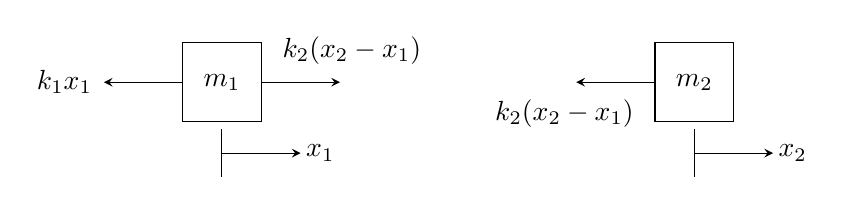
\begin{tikzpicture}
      % first mass
      \draw (2,0) rectangle (3,1);  % mass
      \node at (2.5,0.5) {$m_{1}$};  % mass label
      \draw (2.5, -0.1) -- (2.5, -0.7);  % reference line 
      \draw[->, -{stealth}] (2.5, -0.4) -- (3.5, -0.4);  % coordinate arrow 
      \node at (3.75, -0.4) {$x_{1}$};  % coordinate label
      
      % spring force to left 
      \draw[->, -{stealth}] (2, 0.5) -- (1, 0.5);  % spring force arrow 
      \node at (0.5,0.5) {$k_{1}x_{1}$};  % spring force label
      % spring force to right
      \draw[->, -{stealth}] (3, 0.5) -- (4, 0.5);  % spring force arrow
      \node at (4.15,0.9) {$k_{2}(x_{2} - x_{1})$};  % spring force label

      % second mass
      \draw (8,0) rectangle (9,1);  % mass
      \node at (8.5,0.5) {$m_{2}$};  % mass label
      \draw (8.5, -0.1) -- (8.5, -0.7);  % reference lines
      \draw[->, -{stealth}] (8.5, -0.4) -- (9.5, -0.4);  % coordinate arrow
      \node at (9.75, -0.4) {$x_{2}$};  % coordinate label
      
      % spring force to left
      \draw[->, -{stealth}] (8, 0.5) -- (7, 0.5);  % spring force arrow
      \node at (6.85,0.1) {$k_{2}(x_{2} - x_{1})$};  % spring force label
    \end{tikzpicture}
    \caption{Free-body diagrams of each mass in the system of~\cref{fig:simple_2_dof_model_of_two_masses_connected_in_series_by_two_springs} indicating the restoring force provided by the springs.}\label{fig:fbd_of_two_sprint_mass_system}
  \end{figure}

  Summing forces on each mass in the horisontal direction yields:

  \begin{equation}
    \begin{aligned}
      m_{1}\ddot{x}_{1} &= -k_{1}x_{1} + k_{2}(x_{2} - x_{1}) \\
      m_{2}\ddot{x}_{2} &= -k_{2}(x_{2} - x_{1}),
    \end{aligned}
  \end{equation}

  \noindent Rearranging the equations above yields:

  \begin{equation}
    \label{eq:two_dof_system_of_equations}
    \begin{aligned}
      m_{1}\ddot{x}_{1} + (k_{1} + k_{2}) x_{1} - k_{2}x_{2}  &= 0 \\
      m_{2}\ddot{x}_{2} - k_{2}x_{1} + k_{2}x_{2} &= 0.
    \end{aligned}
  \end{equation}

  \Cref{eq:two_dof_system_of_equations} consist of two coupled second-order ordinary differential equations with constant coefficients, each of which requires two initial conditions to solve. Hence these two coupled equations are subject to the four initial conditions:

  \begin{equation}
    \label{eq:two_dof_initial_conditions}
    \begin{aligned}
      x_{1}(0) &= x_{10} \\
      \dot{x}_{1}(0) &= \dot{x}_{10} \\
      x_{2}(0) &= x_{20} \\
      \dot{x}_{2}(0) &= \dot{x}_{20},
    \end{aligned}
  \end{equation}

  \noindent where the constants $x_{10}$, $\dot{x}_{10}$, $x_{20}$, and $\dot{x}_{20}$ are the initial displacements and velocities of the two masses. These initial conditions are assumed to be known or given and provide the four constants of integration needed to solve the two second-order-differential equations for the free response of each mass. There are multiple different ways to solve the above equations, however, a convenient method of solving this system is to use vectors and matrices. The vector approach t solving this simple two-DOF problem is also readily extendable to systems with an arbitrary finite number of DOFs and is compatible with computer programming.

  We define the vector $\mathbf{x}(t)$ to be the column vector of consisting of the two responses of interest:

  \begin{equation}
    \mathbf{x}(t) = 
    \begin{bmatrix}
      x_{1}(t) \\
      x_{2}(t)
    \end{bmatrix}.
  \end{equation}




